\documentclass[a4paper]{article}
\usepackage[utf8x]{inputenc}
\usepackage[T1,T2A]{fontenc}
\usepackage[russian]{babel}
\usepackage{hyperref}
\usepackage{indentfirst}
\usepackage{listings}
\usepackage{color}
\usepackage{here}
\usepackage{array}
\usepackage{multirow}
\usepackage{graphicx}
\usepackage[space]{grffile}

\usepackage{caption}
\renewcommand{\lstlistingname}{Программа} % заголовок листингов кода

\usepackage{listings}
\lstset{ %
extendedchars=\true,
keepspaces=true,
language=bash,					% choose the language of the code
basicstyle=\footnotesize,		% the size of the fonts that are used for the code
numbers=left,					% where to put the line-numbers
numberstyle=\footnotesize,		% the size of the fonts that are used for the line-numbers
stepnumber=1,					% the step between two line-numbers. If it is 1 each line will be numbered
numbersep=5pt,					% how far the line-numbers are from the code
backgroundcolor=\color{white},	% choose the background color. You must add \usepackage{color}
showspaces=false				% show spaces adding particular underscores
showstringspaces=false,			% underline spaces within strings
showtabs=false,					% show tabs within strings adding particular underscores
frame=single,           		% adds a frame around the code
tabsize=2,						% sets default tabsize to 2 spaces
captionpos=b,					% sets the caption-position to bottom
breaklines=true,				% sets automatic line breaking
breakatwhitespace=false,		% sets if automatic breaks should only happen at whitespace
escapeinside={\%*}{*)},			% if you want to add a comment within your code
postbreak=\raisebox{0ex}[0ex][0ex]{\ensuremath{\color{red}\hookrightarrow\space}}
}

\usepackage[left=2cm,right=2cm,
top=2cm,bottom=2cm,bindingoffset=0cm]{geometry}



\begin{document}	% начало документа

\begin{titlepage}	% начало титульной страницы

	\begin{center}		% выравнивание по центру

		\large Санкт-Петербургский Политехнический Университет Петра Великого\\
		\large Институт компьютерных наук и технологий \\
		\large Кафедра компьютерных систем и программных технологий\\[6cm]
		% название института, затем отступ 6см
		
		\huge Методы и средства защиты информации\\[0.5cm] % название работы, затем отступ 0,5см
		\large Отчет по лабораторной работе №3\\[0.1cm]
		\large Инструмент тестов на проникновение Metasploit\\[5cm]

	\end{center}


	\begin{flushright} % выравнивание по правому краю
		\begin{minipage}{0.25\textwidth} % врезка в половину ширины текста
			\begin{flushleft} % выровнять её содержимое по левому краю

				\large\textbf{Работу выполнил:}\\
				\large Косолапов С.А.\\
				\large {Группа:} 53501/3\\
				
				\large \textbf{Преподаватель:}\\
				\large Вылегжанина К.Д.

			\end{flushleft}
		\end{minipage}
	\end{flushright}
	
	\vfill % заполнить всё доступное ниже пространство

	\begin{center}
	\large Санкт-Петербург\\
	\large \the\year % вывести дату
	\end{center} % закончить выравнивание по центру

\thispagestyle{empty} % не нумеровать страницу
\end{titlepage} % конец титульной страницы

\vfill % заполнить всё доступное ниже пространство


% Содержание
\tableofcontents
\newpage



\section{Цель работы}

Изучить возможности и способы работы с инструментом тестов на проникновение Metasploit. Ознакомиться с консольной и GUI-версиями программного средства и особенностями работы с ними.

\section{Программа работы}

\textbf{Изучение}

\begin{enumerate}

\item Используя документацию изучить базовые понятия - auxiliary, payload, exploit, shellcode, nop, encoder

\item Запустить msfconsole, узнать список допустимых команд (help)

\item Базовые команды search (поиск по имени, типу, автору и др.), info, load, use

\item Команды по работе с эксплойтом

\item Команды по работе с БД

\item GUI оболочка Armitage

\item GUI веб-клиент

\end{enumerate}

\textbf{Практическое задание}

Описать последовательность действий для выполения следующих задач:

\begin{enumerate}

\item Подключиться к VNC-серверу, получить доступ к консоли

\item Получить список директорий в общем доступе по протоколу SMB

\item Получить консоль используя уязвимость в vsftpd

\item Получить консоль используя уязвимость в irc

\item Armitage Hail Mary

\end{enumerate}

Изучить три файла с исходным кодом эксплойтов или служебных скриптов на ruby и описать, что в них происходит.

\section{Теоретическая информация}

\subsection{Используя документацию изучить базовые понятия - auxiliary, payload, exploit, shellcode, nop, encoder}

\begin{itemize}
\item \textbf{auxiliary} ("помощник") - сканер, позволяющий с использованием уязвимостей на атакуемом сервере получать некую вспомогательную информацию.

\item \textbf{payload} - функциональная часть вируса; часть программы, выполняющая вредоносные действия - к примеру, нарушение целостности данных, слежка за пользователем и т.д.

\item \textbf{exploit} - фрагмент програмного кода который, используя возможности предоставляемые ошибкой, отказом или уязвимостью, ведёт к повышению привилегий или отказу в обслуживании компьютерной системы.
			
\item \textbf{shellcode} - двоичный исполняемый код, который обычно передаёт управление командному процессору, например '/bin/sh' в Unix shell, 'command.com' в MS-DOS и 'cmd.exe' в операционных системах Microsoft Windows. Шелл-код может быть использован как полезная нагрузка эксплойта, обеспечивающая взломщику доступ к командной оболочке в компьютерной системе.

\item \textbf{nop} - инструкция процессора на языке ассемблера, или команда протокола, которая предписывает ничего не делать (от слова <<no operation>>). Успешно может быть заменена вредоносными инструкциями. Причём в качестве nop-команды может быть выбрана любая команда, которая не помешает работе эксплойта.
			
\item \textbf{encoder} - преобразователь payload'а в закодированное состояние, необходимое для осуществления конкретной атаки. В частности, могут экранироваться символы, видоизменяться команды и так далее.

\end{itemize}

\subsection{Запустить msfconsole, узнать список допустимых команд (help)}

Все команды делятся на "команды ядра" (core commands) и команды базы данных ("database backend commands"). Команды ядра частично образованы обычными Unix-командами (cd, kill, jobs, help и так далее), а также специфическими командами системы Metasploit, среди которых:

\begin{itemize}

\item back - уйти назад из текущего контекста

\item go\_pro - показать GUI Metasploit

\item и так далее

\end{itemize}

Полный список команд: 

\lstinputlisting[numbers=none, keywords={}]{logs/help.txt}

\subsection{Базовые команды search (поиск по имени, типу, автору и др.), info, load, use}

\begin{itemize}

\item \textbf{search} - поиск модуля и его описания

\item \textbf{info} - вывод информации о модуле/полезной нагрузке

\item \textbf{load} - загрузить плагин фреймворка

\item \textbf{use} - выбрать модуль для последующего использования

\end{itemize}

\subsection{Команды по работе с эксплойтом}

\begin{itemize}
\item \textbf{show options} - просмотреть параметры для настройки. После выбора эксплойта можно просмотреть, какие опции доступны для настройки.

\item \textbf{show payload} - просмотреть полезные нагрузки. В частности, может быть получена рекомендация полезных нагрузок для данного эксплойта или ОС.

\item \textbf{set} - установить параметры, либо полезную нагрузку

\item \textbf{check} - проверить на уязвимость

\item \textbf{exploit} - запустить эксплойт

\end{itemize}

\subsection{Команды по работе с БД}

Команды управления базой данных, среди прочих, включают в себя:

\begin{itemize}

\item \textbf{db\_connect} - присоединиться к базе данных

\item \textbf{db\_import} - импортировать результат сканирования

\item \textbf{db\_status} - показать текущий статус базы данных

\item \textbf{services} - показать сервисы базы данных

\item \textbf{workspace} - переключиться между рабочими областями

\item ...

\end{itemize}

\subsection{GUI оболочка Armitage}

Графическая оболочка Armitage являет собой фронтенд для фреймворка Metasploit и за счёт визуального представления позволяет лучше понять процесс атаки.

\begin{figure}[H]
	\begin{center}
		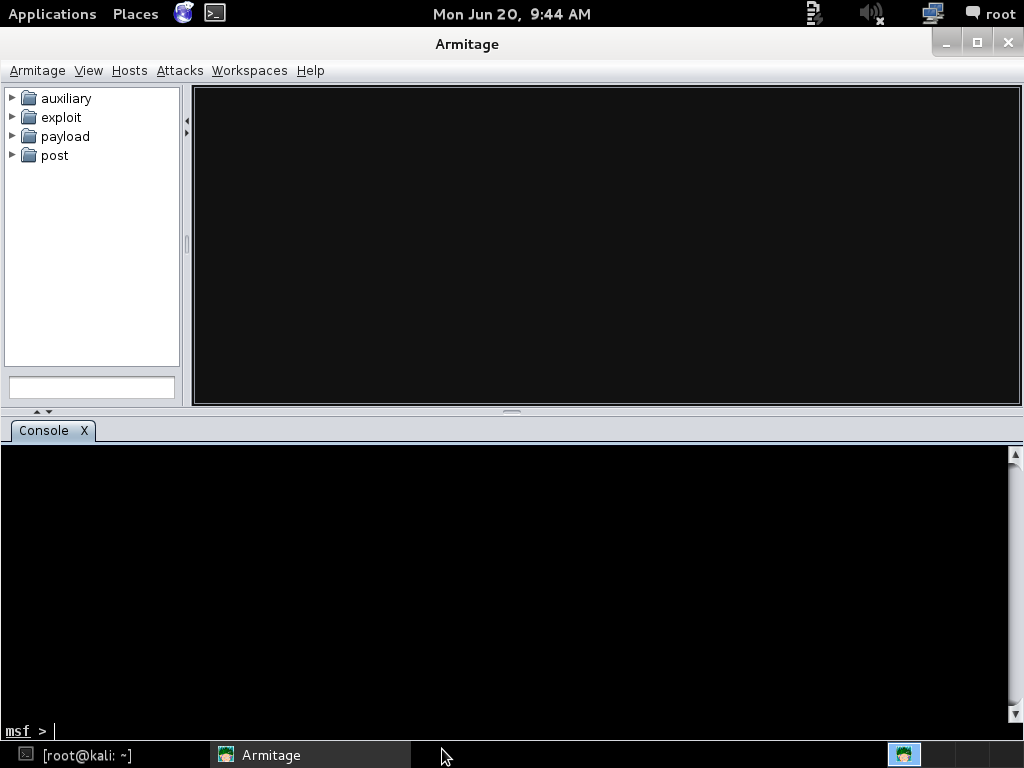
\includegraphics[scale=0.5]{pics/armitage.png}
		\caption{Оболочка Armitage} 
		\label{pic:pic_name}
	\end{center}
\end{figure}

\subsection{GUI веб-клиент}

Для доступа к клиенту необходимо проверить статус веб-сервера Metasploit и запустить сервис Apache. Клиент будет доступен по адресу 3790.

\section{Ход выполнения работы}

\subsection{Провести поиск активных хостов}

Поиск производим с помощью утилиты nmap из msfconsole:

\lstinputlisting[numbers=none, keywords={}]{logs/scan.txt}

\subsection{Подключиться к VNC-серверу, получить доступ к консоли}

Сначала с помощью команды \textbf{search} найдём нужный модуль:

\lstinputlisting[numbers=none, keywords={}, lastline=55]{logs/vnc_msf.txt}

Затем выберем auxiliary с помощью \textbf{use}, а также установим хост и количество потоков:

\lstinputlisting[numbers=none, keywords={}, firstline=62, lastline=66]{logs/vnc_msf.txt}

Затем запустим auxiliary:

\lstinputlisting[numbers=none, keywords={}, firstline=67]{logs/vnc_msf.txt}

Как видим, получили пароль. Теперь можем его подставить:

\lstinputlisting[numbers=none, keywords={}]{logs/vnc_result.txt}

C паролем успешно прошли аутентификацию.

\begin{figure}[H]
	\begin{center}
		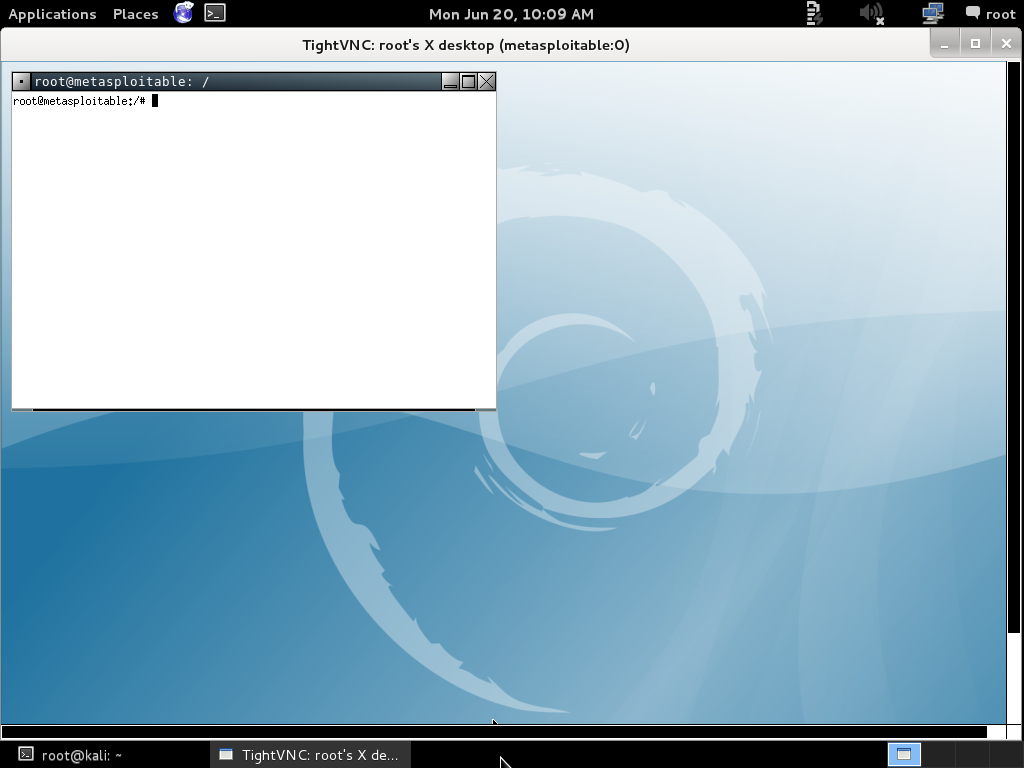
\includegraphics[scale=0.5]{pics/tightvnc.png}
		\caption{Запущенный GUI TightVNC} 
		\label{pic:pic_name}
	\end{center}
\end{figure}

\subsection{Получить список директорий в общем доступе по протоколу SMB}

Сначала ищем модуль, который поможет нам это сделать:

\lstinputlisting[numbers=none, keywords={}, lastline=1]{logs/smb_msf.txt}

Среди довольно длинного списка находим нужный:

\lstinputlisting[numbers=none, keywords={}, firstline=49, lastline=49]{logs/smb_msf.txt}

Далее выбираем модуль и устанавливаем параметры:

\lstinputlisting[numbers=none, keywords={}, firstline=99, lastline=103]{logs/smb_msf.txt}

Запускаем auxiliary:

\lstinputlisting[numbers=none, keywords={}, firstline=104]{logs/smb_msf.txt}

В результате видим список директорий, находящихся в общем доступе.

\subsection{Получить консоль используя уязвимость в vsftpd}

Сначала найдём модуль:

\lstinputlisting[numbers=none, keywords={}, lastline=8]{logs/vsftpd_msf.txt}

Затем активируем модуль и установим хост:

\lstinputlisting[numbers=none, keywords={}, firstline=11, lastline=13]{logs/vsftpd_msf.txt}

После чего можем использовать эксплойт:

\lstinputlisting[numbers=none, keywords={}, firstline=14]{logs/vsftpd_msf.txt}

Как видим, с помощью уязвимости сумели получить доступ к консоли от имени суперпользователя.

Странно, но команда `who am i` не работает.

\subsection{Получить консоль используя уязвимость в irc}

Посмотрим версию сервиса:

\lstinputlisting[numbers=none, keywords={}, lastline=14]{logs/irc_msf.txt}

Затем найдём эксплойт для данной версии:

\lstinputlisting[numbers=none, keywords={}, firstline=16, lastline=25]{logs/irc_msf.txt}

После этого выберем модуль эксплойта и установим настройки:

\lstinputlisting[numbers=none, keywords={}, firstline=28, lastline=34]{logs/irc_msf.txt}

Теперь можем использовать эксплойт на удалённой машине:

\lstinputlisting[numbers=none, keywords={}, firstline=35]{logs/irc_msf.txt}

Таким образом, мы получили доступ к консоли удалённого хоста. Мало того, доступ получили под рутом. Для примера использования уязвимости был создан файл в каталоге /home/msfadmin.

\begin{figure}[H]
	\begin{center}
		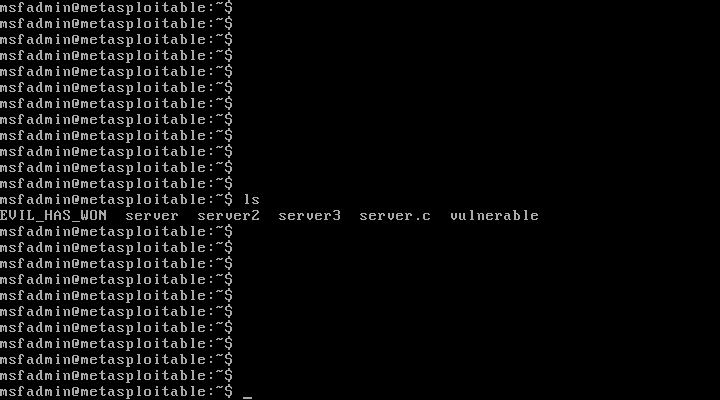
\includegraphics[scale=0.5]{pics/evilhaswon.png}
		\caption{Файлы в директории /home/msfadmin атакованного хоста} 
		\label{pic:pic_name}
	\end{center}
\end{figure}

\subsection{Armitage Hail Mary}

В программе Armitage - графической оболочке для Metasploit - есть множество возможностей по автоматизированному сканированию и применению различных атак. Наиболее интересной является возможность, называемая Hail Mary, которая заключается в полном сканировании, внедрении payload'ов, запуска подходящих эксплойтов. Таким образом, производится "умная" автоматизированная атака на удалённый хост.


Если armitage найдёт хост, либо мы вручную укажем его, то GUI будет выглядеть примерно следующим образом:

\begin{figure}[H]
	\begin{center}
		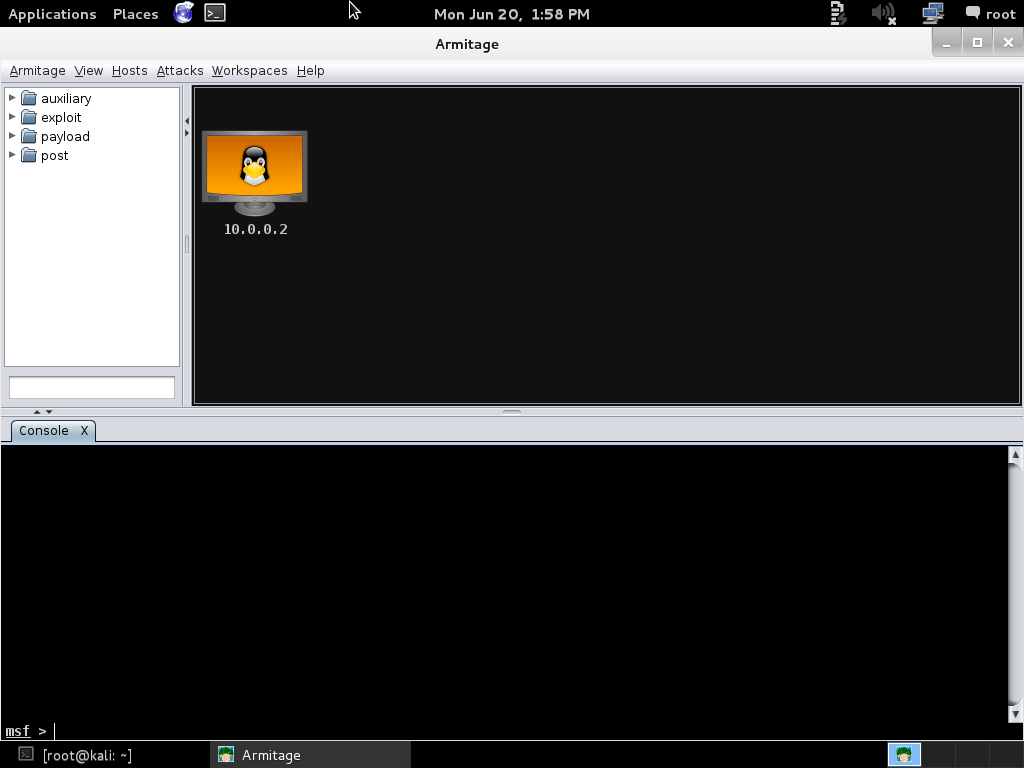
\includegraphics[scale=0.5]{pics/armitage_host_found.png}
		\caption{Armitage с найденным хостом} 
		\label{pic:pic_name}
	\end{center}
\end{figure}

В данном примере рассматривалась атака на один хост, но их может быть много.

Далее можно просканировать хост на наличие уязвимостей:

\lstinputlisting[numbers=none, keywords={}]{logs/armitage_scan.txt}

После этого можно запустить Hail Mary. В результате получим примерно следующую картинку:

\begin{figure}[H]
	\begin{center}
		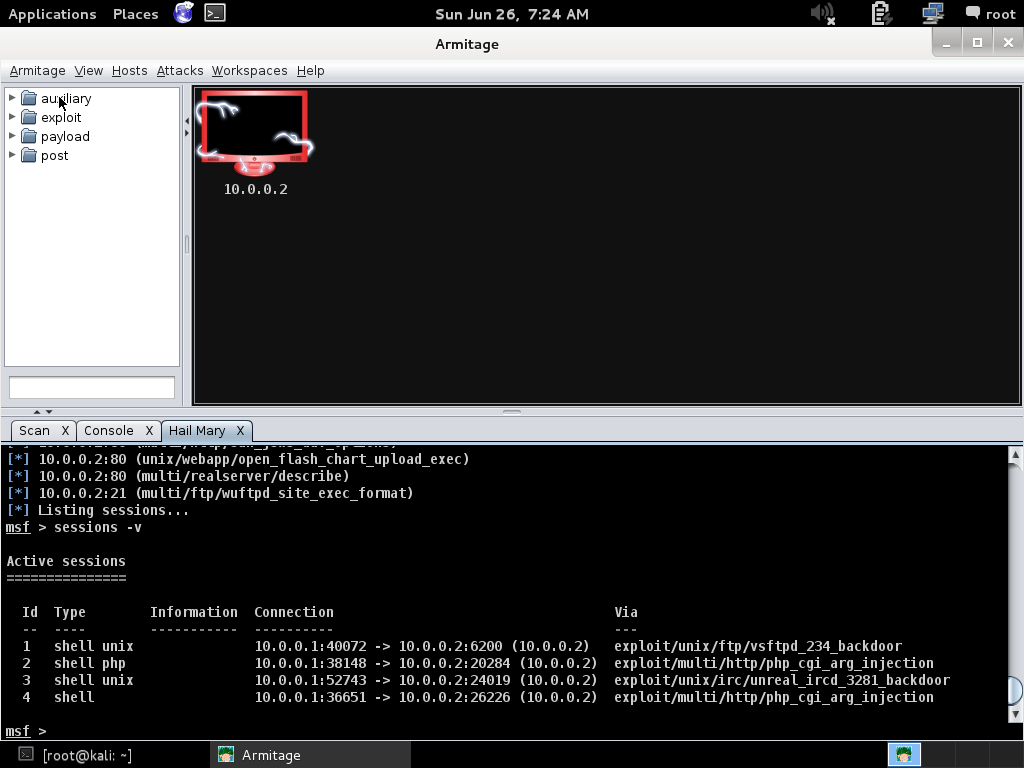
\includegraphics[scale=0.5]{pics/armitage_attacked.png}
		\caption{Атакованный хост в Armitage} 
		\label{pic:pic_name}
	\end{center}
\end{figure}

Стоит отметить, что после первого запуска Hail Mary было зафиксировано использование только двух уязвимостей, а после второго - четырёх, среди которых одна дублируется. Возможно, это связано с довольно медленной работой виртуальной машины.

\subsection{Изучить три файла с исходным кодом эксплойтов или служебных скриптов на ruby и описать, что в них происходит}

Тексты исходных кодов были взяты из репозитория Metasploit Framework (https://github.com/rapid7/metasploit-framework/).

\subsubsection{/modules/nops/php/generic.rb}

\lstinputlisting[language=ruby]{code/php_generic.rb}

Довольно простой модуль. Класс наследуется от Msf::Nop, перегружается функция Initialize, где указываются параметры скрипта, а также функция generate\_sled. Для интерпретируемого языка достаточно прописать пробелы, в которые затем можно внедрить вредоносный код.

\subsubsection{.modules/auxiliary/scanner/http/ssl.rb}

\lstinputlisting[language=ruby]{code/ssl.rb}

Подробно действия описаны в комментариях к коду. Если кратко, то мы соединяемся, получаем сертификат, после чего отсоединяемся. Далее анализируем различные уязвимости в сертификате и настраиваем окружение для работы с этим сертификатом.

\subsection{/modules/exploits/unix/ftp/vsftpd\_234\_backdoor.rb}

\lstinputlisting[language=ruby]{code/vsftpd_234_backdoor.rb}

Подробные комментарии описаны в коде. Кратко \- сначала проверяем, не задействован ли бэкдор уже. Если нет \- посылаем случайную последовательность с префиксом "USER: ", затем случайную последовательность с префиксом "PASS: ". В результате, можем подключиться к удалённому хосту. Далее вызывается функция handle\_backdoor, в которой проверяется, является ли сервис консолью, а затем вызывается стандартный обработчик удалённой консоли.

\section{Выводы}

Пакет Metasploit Framework предоставляет огромные возможности для достаточно простого сканирования удалённых хостов и поиска уязвимостей. Он включает в себя несколько разделов, среди которых auxiliary, payload, exploit, nop и другие. Первый предназначен для поиска информации определённого типа об удалённой системе, предназначенную, в первую очередь, для проведения последующих атак. Другие - для использования уязвимостей с целью получения доступа, повышения прав, проведения определённых операций над данными на удалённой машине и так далее. Тот или иной компонент раздела является скриптом и написан на языке Ruby, можно простыми средствами дополнять их набор и использовать новые для проведения атак.

Отдельно стоит отметить графическую оболочку Armitage, которая позволяет максимально упростить процесс сканирования удалённых узлов и проведения атак. Так, Armitage Hail Mary позволяет найти уязвимости, содержащиеся в базе, и задействовать их, что, благодаря графической оболочке, можно сделать в два клика.

\end{document}